\PassOptionsToPackage{unicode}{hyperref}
\documentclass[aspectratio=1610, professionalfonts, 9pt]{beamer}

\usefonttheme[onlymath]{serif}
\usetheme[showtotalframes]{tudo}

\ifluatex
  \usepackage{polyglossia}
  \setmainlanguage{german}
\else
  \ifxetex
    \usepackage{polyglossia}
    \setmainlanguage{german}
  \else
    \usepackage[german]{babel}
  \fi
\fi
    

% Mathematik
\usepackage{amsmath}
\usepackage{amssymb}
\usepackage{mathtools}
\usepackage{cancel}

\usepackage{hyperref}
\usepackage{bookmark}

%%%%%%%%%%%%%%%%%%%%%%%%%%%%%%%%%%%%%%%%%%%%%%%%%%%%%%%%%%%%%%%%%%%%%%%%%%%%%%%%
%%%%%-------------Hier Titel/Autor/Grafik/Lehrstuhl eintragen--------------%%%%%
%%%%%%%%%%%%%%%%%%%%%%%%%%%%%%%%%%%%%%%%%%%%%%%%%%%%%%%%%%%%%%%%%%%%%%%%%%%%%%%%

%Titel:
\title{\LaTeX-Beamer-Theme der TU~Dortmund}
%Autor
\author[M.~Nöthe]{Maximilian Nöthe}
%Lehrstuhl/Fakultät
\institute[Experimental Physics 5]{Names des Lehrstuhls \\  Name der Fakultät}
%Titelgrafik 
\titlegraphic{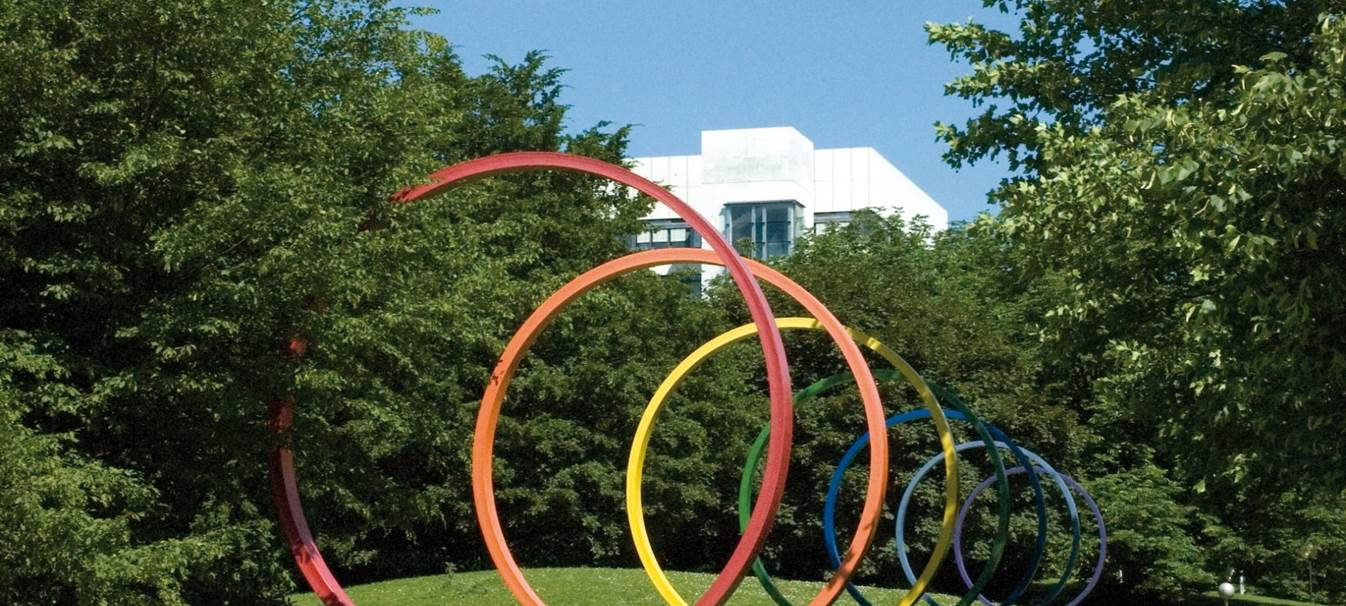
\includegraphics[width=0.7\textwidth]{images/tudo-title-2.jpg}}


\begin{document}

\maketitle

\begin{frame}{Hinweise}
  Zu diesem Theme
  \begin{itemize}
    \item Zur Installation des Themese muss mindestens die Datei \texttt{beamerthemetudo.sty} und der Ordner \texttt{logos} in einen Ordner verschoben werden, in dem \LaTeX nach Paketen sucht.
      Dies können sein
      \begin{itemize}
        \item \texttt{TEXMFHOME/tex/latex/tudobeamertheme}. Den Wert von \texttt{TEXMFHOME} bekommen sie über \texttt{kpsewhich --var-value TEXMFHOME}, üblicherweise ist dies \texttt{\$HOME/texmf}.
        \item Der gleiche Ordner in dem Sie ihr Dokument kompilieren
        \item Ein beliebiger Ordner, der in der Variablen \texttt{TEXINPUTS} enthalten ist.
      \end{itemize}
  \end{itemize}
  Allgemein zu Beamer und Latex:
  \begin{itemize}
    \item Umfangreicher \LaTeX-Kurs von PeP et Al. \\
      \url{http://toolbox.pep-dortmund.org/notes}
    \item Latex-Beamer Dokumetation:\\
    \url{http://www.ctan.org/pkg/beamer}
  \end{itemize}
\end{frame}

\begin{frame}
    \frametitle{Einführung}
    \tableofcontents[pausesections]
\end{frame}

\section{Blindtext}
\begin{frame}
	\frametitle{Hier steht eine lange, zweizeilige Headline
		\newline gefolgt von einem Blindtext}
Dieser Text dient nur zur Veranschaulichung des Textsatzes. Niemand sollte jemals, aus keinem noch so gutem Grund, so viel Text auf eine Folie packen.

Dies ist ein Blindtext. Dieser Text ist nicht dafür vorgesehen, den Betrachter in die Welt der Dunkelheit zu führen, sondern dafür, einfach etwas Leeres mit etwas Inhaltlosem zu füllen.

Dies ist ein Blindtext. Dieser Text ist nicht dafür vorgesehen, den Betrachter in die Welt der Dunkelheit zu führen, sondern dafür, einfach etwas Leeres mit etwas Inhaltlosem zu füllen.

Dies ist ein Blindtext. Dieser Text ist nicht dafür vorgesehen, den Betrachter in die Welt der Dunkelheit zu führen, sondern dafür, einfach etwas Leeres mit etwas Inhaltlosem zu füllen.
\end{frame}

\begin{frame}{title}
  \begin{enumerate}
    \item test
    \item test
  \end{enumerate}
\end{frame}

\begin{frame}{title}
  \begin{block}{title}
    ANlsnldas dkmadföonslkadm x
  \end{block}
\end{frame}
\end{document}
